\documentclass[10pt,compress]{beamer}
\usetheme{Madrid}
\definecolor{aggiemaroon}{RGB}{153,0,51} 
\usecolortheme[named=aggiemaroon]{structure}
\useoutertheme{shadow}
\useinnertheme{rounded}
\setbeamertemplate{navigation symbols}{}
\setbeamerfont{structure}{family=\rmfamily,series=\bfseries}
\usefonttheme[stillsansseriftext]{serif}

\graphicspath{ {./} }
\usepackage{braket}
\usepackage{listings}
\usepackage[qm]{qcircuit}
\newcommand{\modd}{\; mod \;}

\usepackage{amsmath}
\usepackage{caption}
\usepackage{graphicx,comment}
\usepackage[spanish]{babel}
\usepackage{graphicx}
\usepackage{rotating}
\usepackage{multicol}
\usepackage{hyperref}
\usepackage{enumerate}
\usepackage{tikz}
\usepackage{graphicx}
\usefonttheme{professionalfonts}
\usefonttheme{serif}
\usepackage{fontspec}
\setmainfont[
Path=Core/,
BoldFont=1.ttf,
ItalicFont=2.ttf,
BoldItalicFont=3.ttf,
]{4.ttf}
\usepackage{bm}

\usebackgroundtemplate{
\tikz\node[opacity=0.025, rotate = 23] {
\includegraphics[height=1.1\paperheight,width=1.1\paperwidth]{ucm.jpg}};}


\title[Universidad Complutense de Madrid]{Introducción a la Computación Cuántica, Algoritmos e Implementación}

\author [Chenjie]{Chenjie Huang}

\date[\today]{}

\institute[UCM] 
{\emph{Sección Departamental de Sistemas Informáticos y Computación}, Tutor: Luis Fernando Llana Díaz\\[.5 cm]
 
\includegraphics[scale=0.1]{LOGO.png} \\ [0.0 cm]
 }




\begin{document}


\begin{frame}
\titlepage
\end{frame}

\begin{frame}
\frametitle{Índice}
\tableofcontents
\end{frame}

\section{Quantum Bit}

\begin{frame}
\frametitle{Bit Cúantico (Qubit)}

\begin{block}{Quantum Bit}
\begin{itemize}
\item<+-> Puede tomar dos estados clásicos $\ket{0}$ y $\ket{1}$.

\item<+-> O cualquier combinación de ellas:
	\begin{equation}
	\ket{\varphi} = \alpha\ket{0} + \beta\ket{1} \; \alpha, \beta \in \mathbb{C}
	\end{equation}
	donde $|\alpha|^2 + |\beta|^2 = 1$.

\uncover<+->{
\begin{center}
\scalebox{0.7}{
\centering

\tikzset{every picture/.style={line width=0.75pt}} %set default line width to 0.75pt        

\begin{tikzpicture}[x=0.75pt,y=0.75pt,yscale=-0.5,xscale=0.5]
%uncomment if require: \path (0,300); %set diagram left start at 0, and has height of 300

%Shape: Circle [id:dp931798172156461] 
\draw   (198,152.5) .. controls (198,90.92) and (247.92,41) .. (309.5,41) .. controls (371.08,41) and (421,90.92) .. (421,152.5) .. controls (421,214.08) and (371.08,264) .. (309.5,264) .. controls (247.92,264) and (198,214.08) .. (198,152.5) -- cycle ;
%Straight Lines [id:da9642706265204986] 
\draw  [dash pattern={on 0.84pt off 2.51pt}]  (198,152.5) -- (421,152.5) ;
%Straight Lines [id:da48160384496840947] 
\draw  [dash pattern={on 0.84pt off 2.51pt}]  (309.5,264) -- (309.5,41) ;
%Straight Lines [id:da8747207133103256] 
\draw    (309.5,152.5) -- (419,152.5) ;
\draw [shift={(421,152.5)}, rotate = 180] [color={rgb, 255:red, 0; green, 0; blue, 0 }  ][line width=0.75]    (10.93,-3.29) .. controls (6.95,-1.4) and (3.31,-0.3) .. (0,0) .. controls (3.31,0.3) and (6.95,1.4) .. (10.93,3.29)   ;
%Straight Lines [id:da7616528840577454] 
\draw    (309.5,152.5) -- (390.28,76.17) ;
\draw [shift={(391.73,74.8)}, rotate = 136.62] [color={rgb, 255:red, 0; green, 0; blue, 0 }  ][line width=0.75]    (10.93,-3.29) .. controls (6.95,-1.4) and (3.31,-0.3) .. (0,0) .. controls (3.31,0.3) and (6.95,1.4) .. (10.93,3.29)   ;
%Straight Lines [id:da30485545720038276] 
\draw    (309.5,152.5) -- (309.5,43) ;
\draw [shift={(309.5,41)}, rotate = 90] [color={rgb, 255:red, 0; green, 0; blue, 0 }  ][line width=0.75]    (10.93,-3.29) .. controls (6.95,-1.4) and (3.31,-0.3) .. (0,0) .. controls (3.31,0.3) and (6.95,1.4) .. (10.93,3.29)   ;

% Text Node
\draw (402,59.93) node [anchor=north west][inner sep=0.75pt]    {$|\varphi \rangle $};
% Text Node
\draw (299.33,5.93) node [anchor=north west][inner sep=0.75pt]    {$|1\rangle $};
% Text Node
\draw (429.33,144.6) node [anchor=north west][inner sep=0.75pt]    {$|0\rangle $};

\end{tikzpicture}}
\end{center}}
\end{itemize}
\end{block}

\end{frame}

\begin{frame}
\frametitle{Bit Cúantico (Qubit)}

\begin{block}{Esfera de Bloch}
Otra forma de representarlo es con coordenadas polares en una esfera.
\begin{equation}
\ket{\psi} = \cos \theta \ket{0} + e^{i\varphi} \sin \theta \ket{1}
\end{equation}

\uncover<2->{
\begin{center}
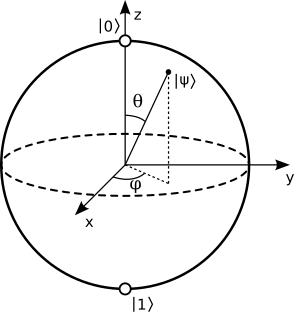
\includegraphics[scale=0.7]{esfera_bloch}
\end{center}
}
\end{block}

\end{frame}

\section{Puertas cuánticas}

\begin{frame}{Puertas Cuánticas}

Puerta $NOT$ (Pauli $X$): \qquad $\Qcircuit{&\gate{X}&\qw}$
\begin{equation}
\begin{cases}
\ket{0} \longrightarrow \ket{1} \\
\ket{1} \longrightarrow \ket{0}
\end{cases}
\end{equation}
\pause
Representación Matricial:
\begin{equation}
\ket{0} =
\begin{bmatrix}
1 \\ 0
\end{bmatrix}, \;
\ket{1} =
\begin{bmatrix}
0 \\ 1
\end{bmatrix}, \;
X =
\begin{bmatrix}
0 & 1 \\
1 & 0 
\end{bmatrix}
\end{equation}
\pause
\begin{equation}
\begin{bmatrix}
0 & 1 \\
1 & 0 
\end{bmatrix}
\only<3>{
\begin{bmatrix}
1 \\ 0
\end{bmatrix}}
\only<4->{\ket{0}} =
\only<3>{
\begin{bmatrix}
0 \\ 1
\end{bmatrix}}
\only<4->{\ket{1}}
\qquad
\begin{bmatrix}
0 & 1 \\
1 & 0 
\end{bmatrix}
\only<3,4>{
\begin{bmatrix}
0 \\ 1
\end{bmatrix}}
\only<5->{\ket{1}} =
\only<3,4>{
\begin{bmatrix}
1 \\ 0
\end{bmatrix}}
\only<5->{\ket{0}}
\end{equation}

\end{frame}

\begin{frame}{Puertas Cuánticas}
Puerta controlada $NOT$ ($CNOT$):
\begin{center}
\scalebox{1.0}{
\Qcircuit @C=1.0em @R=0.8em @!R {
	 \lstick{\ket{x}} & \ctrl{1} & \rstick{\ket{x}} \qw \\
	 \lstick{\ket{y}} & \targ & \rstick{\ket{x\oplus y}} \qw}}
\end{center}
\pause
\begin{equation}
\only<2>{
\begin{cases}
\ket{0}\otimes\ket{0} \rightarrow \ket{0}\otimes\ket{0} \\
\ket{0}\otimes\ket{1} \rightarrow \ket{0}\otimes\ket{1}
\end{cases}
\qquad
\begin{cases}
\ket{1}\otimes\ket{0} \rightarrow \ket{1}\otimes\ket{1} \\
\ket{1}\otimes\ket{1} \rightarrow \ket{1}\otimes\ket{0}
\end{cases}}
\only<3->{
\begin{cases}
\ket{00} \rightarrow \ket{00} \\
\ket{01} \rightarrow \ket{01}
\end{cases}
\qquad
\begin{cases}
\ket{10} \rightarrow \ket{11} \\
\ket{11} \rightarrow \ket{10}
\end{cases}}
\end{equation}
\uncover<4->{
\begin{equation}
CNOT
\ket{10}
= \begin{bmatrix}
1 & 0 & 0 & 0 \\
0 & 1 & 0 & 0 \\
0 & 0 & 0 & 1 \\
0 & 0 & 1 & 0 
\end{bmatrix}
\only<4>{
\begin{bmatrix}
0 \\ 0 \\ 1 \\ 0
\end{bmatrix}}
\only<5>{
\begin{bmatrix}
0 \\ 1
\end{bmatrix}\otimes
\begin{bmatrix}
1 \\ 0
\end{bmatrix}}
\only<6->{\ket{1}\otimes\ket{0}} =
\only<4>{
\begin{bmatrix}
0 \\ 0 \\ 0 \\ 1
\end{bmatrix}}
\only<5>{
\begin{bmatrix}
0 \\ 1
\end{bmatrix}\otimes
\begin{bmatrix}
0 \\ 1
\end{bmatrix}}
\only<6->{\ket{1}\otimes\ket{1}}
\end{equation}}

\end{frame}

\section{Algoritmos cuánticos}

\begin{frame}{Algoritmo de Teletransportación}
\begin{center}
\scalebox{1.5}{
\Qcircuit @C=1.0em @R=0.2em @!R { \\
	 	\rstick{\ket{\varphi}} & \nghost{} & \ctrl{1} & \gate{\mathrm{H}} & \meter & \cw & \controlo \cw_(0.4){\mathrm{M_1}} \cwx[2] \\
	 	\dstick{\ket{\beta_{00}}} & \nghost{} & \targ & \qw & \meter & \controlo \cw_(0.4){\mathrm{M_2}} \cwx[1]  \\
	 	\nghost{} & \nghost{} & \qw & \qw & \qw & \gate{\mathrm{Z^{M_2}}} & \gate{\mathrm{X^{M_1}}} & \qw &\rstick{\ket{\varphi}}\\}}
\end{center}
\end{frame}

\begin{frame}{Algoritmo de Deutsch}
\begin{block}{Oráculo}
El oráculo es una operación unitaria $U_f$ que nos permitirá evaluar una función $f:\{0,1\}^n \longrightarrow \{0,1\}^n$.
\begin{center}
\scalebox{1.5}{
\Qcircuit @C=1.0em @R=0.8em @!R {
	 \lstick{\ket{x}} & \multigate{1}{\hspace{0.2cm}\mathrm{U_f}\hspace{0.2cm}} & \rstick{\ket{x}} \qw \\
	 \lstick{\ket{y}} & \nghost{\hspace{0.2cm}\mathrm{U_f}\hspace{0.2cm}} \qw & \rstick{\ket{y\oplus f(x)}} \qw}}
\end{center}
\end{block}
\pause
Circuito para el algoritmo de Deutsch:
\begin{center}
\scalebox{1.5}{
\Qcircuit @C=1.0em @R=0.8em @!R {
	 \nghost{} & \qw_(0.0){\ket{0}} & \gate{\mathrm{H}} & \qw & \multigate{1}{\hspace{0.2cm}\mathrm{U_f}\hspace{0.2cm}} & \qw & \gate{\mathrm{H}} & \qw & \meter \\
	 \nghost{} & \qw_(0.0){\ket{1}} & \gate{\mathrm{H}} & \qw & \nghost{\hspace{0.2cm}\mathrm{U_f}\hspace{0.2cm}} \qw & \qw & \qw & \qw & \qw}}
\end{center}

\end{frame}

\begin{frame}[fragile]{Algoritmo de Deutsch}
\begin{columns}
\column{0.5\textwidth}

\begin{lstlisting}[language=Python]
circ = QuantumCircuit(2, 1)
circ.x(1)
circ.h(range(2))
gf = Operator([[0,0,1,0],
               [0,1,0,0],
               [1,0,0,0],
               [0,0,0,1]])
circ.append(gf, [0,1])
circ.h(0)
circ.barrier(range(2))
circ.measure(range(1),range(1))
circ.draw('mpl')
\end{lstlisting}

\column{0.5\textwidth}
\begin{center}
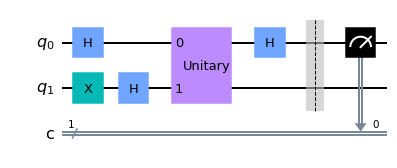
\includegraphics[height=10em,width=\hsize]{qc_deutsch}
\end{center}

\end{columns}

\end{frame}

\begin{frame}{Algoritmo de Deutsch-Jozsa}
Circuito para el algoritmo de Deutsch-Jozsa:
\begin{center}
\scalebox{1.3}{
\Qcircuit @C=1.0em @R=0.8em @!R {
	 \nghost{} & \rstick{/^{n}} \qw_(0.0){\ket{\mathbf{0}}} & \qw & \gate{\mathrm{H}^{\otimes n}} & \qw & \lstick{/^{n}} \qw & \multigate{1}{\hspace{0.3cm}\mathrm{U_f}\hspace{0.3cm}} & \qw & \lstick{/^{n}} \qw & \gate{\mathrm{H^{\otimes n}}} & \qw & \lstick{/^{n}} \qw & \meter \\
	 \nghost{} & \qw_(0.0){\ket{1}} & \qw & \gate{\mathrm{H}} & \qw & \qw & \nghost{\hspace{0.3cm}\mathrm{U_f}\hspace{0.3cm}} \qw & \qw & \qw & \qw & \qw & \qw & \qw \\}}
\end{center}

\end{frame}

\begin{frame}[fragile]{Algoritmo de Deutsch-Jozsa}
\begin{columns}
\column{0.5\textwidth}

\begin{lstlisting}[language=Python]
circ = QuantumCircuit(3,2)
circ.x(2)
circ.h(range(3))
gf = Operator(
    [[1,0,0,0,0,0,0,0],
    [0,0,0,0,0,1,0,0],
    [0,0,1,0,0,0,0,0],
    [0,0,0,0,0,0,0,1],
    [0,0,0,0,1,0,0,0],
    [0,1,0,0,0,0,0,0],
    [0,0,0,0,0,0,1,0],
    [0,0,0,1,0,0,0,0]])
circ.append(gf, [0,1,2])
circ.h(range(2))
circ.barrier(range(3))
circ.measure(range(2),range(2))
circ.draw('mpl')
\end{lstlisting}

\column{0.5\textwidth}
\begin{center}
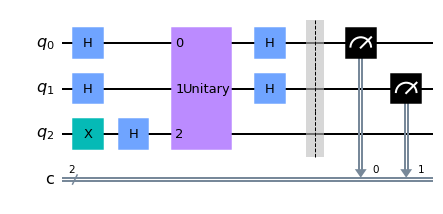
\includegraphics[width=\hsize]{qc_deutsch_jozsa}
\end{center}

\end{columns}

\end{frame}

\begin{frame}{Algoritmo de Búsqueda de Grover}
Circuito para el algoritmo de Grover:
\begin{center}
\scalebox{1.0}{
\Qcircuit @C=1.0em @R=0.8em @!R {
	 \nghost{} & \rstick{/^{n}} \qw_(0.0){\ket{\mathbf{0}}} & \qw & \gate{\mathrm{H}^{\otimes n}} & \qw & \lstick{/^{n}} \qw & \multigate{1}{\hspace{0.3cm}\mathrm{U_f}\hspace{0.3cm}} & \qw & \lstick{/^{n}} \qw & \gate{\mathrm{H^{\otimes n}}} & \gate{2\ket{\mathbf{0}}\bra{\mathbf{0}} - I} & \gate{\mathrm{H^{\otimes n}}} & \qw & \lstick{/^{n}} \qw & \meter \\
	 \nghost{} & \qw_(0.0){\ket{1}} & \qw & \gate{\mathrm{H}} & \qw & \qw & \nghost{\hspace{0.3cm}\mathrm{U_f}\hspace{0.3cm}} \qw & \qw & \qw & \qw & \qw & \qw & \qw & \qw & \qw
	 \gategroup{1}{7}{2}{12}{0.7em}{--}
}}
\end{center}
\end{frame}

\begin{frame}{Algoritmo de Búsqueda de Grover}
Representación geométrica:

\begin{center}

\begin{tikzpicture}[x=0.75pt,y=0.75pt,yscale=-0.6,xscale=0.6]
%uncomment if require: \path (0,369); %set diagram left start at 0, and has height of 369

\uncover<1->{
%-Eje
%Shape: Axis 2D [id:dp7055697676389285] 
\draw  (169.2,241.7) -- (410.24,241.7)(192.62,25.6) -- (192.62,264.07) (403.24,236.7) -- (410.24,241.7) -- (403.24,246.7) (187.62,32.6) -- (192.62,25.6) -- (197.62,32.6)  ;
% Text Node
\draw (416.4,231) node [anchor=north west][inner sep=0.75pt]   [align=left] {$\displaystyle |\alpha \rangle $};
% Text Node
\draw (160.4,21.6) node [anchor=north west][inner sep=0.75pt]   [align=left] {$\displaystyle |\beta \rangle $};

%ket psi
%Straight Lines [id:da0346206509250393] 
\draw    (192.62,241.7) -- (397.91,200.53) ;
\draw [shift={(399.87,200.13)}, rotate = 168.66] [color={rgb, 255:red, 0; green, 0; blue, 0 }  ][line width=0.75]    (10.93,-3.29) .. controls (6.95,-1.4) and (3.31,-0.3) .. (0,0) .. controls (3.31,0.3) and (6.95,1.4) .. (10.93,3.29)   ;
% Text Node
\draw (405.33,180.6) node [anchor=north west][inner sep=0.75pt]    {$|\psi \rangle $};
}


\uncover<2->{
%simetria1
%Straight Lines [id:da46392021083734325] 
\draw    (192.62,241.7) -- (397.9,280.69) ;
\draw [shift={(399.87,281.07)}, rotate = 190.76] [color={rgb, 255:red, 0; green, 0; blue, 0 }  ][line width=0.75]    (10.93,-3.29) .. controls (6.95,-1.4) and (3.31,-0.3) .. (0,0) .. controls (3.31,0.3) and (6.95,1.4) .. (10.93,3.29)   ;
% Text Node
\draw (409.33,277.93) node [anchor=north west][inner sep=0.75pt]    {$U |\psi \rangle $};
%Straight Lines [id:da3011553594885228] 
\draw  [dash pattern={on 0.84pt off 2.51pt}]  (399.87,281.07) -- (399.87,200.13) ;
}

\uncover<3->{
%simetria2
%Straight Lines [id:da34055073615610354] 
\draw    (192.62,241.7) -- (368.7,131.46) ;
\draw [shift={(370.4,130.4)}, rotate = 147.95] [color={rgb, 255:red, 0; green, 0; blue, 0 }  ][line width=0.75]    (10.93,-3.29) .. controls (6.95,-1.4) and (3.31,-0.3) .. (0,0) .. controls (3.31,0.3) and (6.95,1.4) .. (10.93,3.29)   ;
% Text Node
\draw (376.67,112.47) node [anchor=north west][inner sep=0.75pt]    {$G|\psi \rangle $};

%Straight Lines [id:da8076953012129235] 
\draw  [dash pattern={on 0.84pt off 2.51pt}]  (370.4,130.4) -- (399.87,281.07) ;
}

\uncover<4->{
%angulos
%Curve Lines [id:da9752809394486917] 
\draw    (325.2,215.07) .. controls (334.69,225.22) and (335.2,255.73) .. (326.53,267.07) ;
%Curve Lines [id:da2736382127737216] 
\draw    (309.87,168.4) .. controls (323.47,177.73) and (331.2,198.4) .. (330.53,214.4) ;
% Text Node
\draw (337.33,222.6) node [anchor=north west][inner sep=0.75pt]  [font=\scriptsize]  {$\theta /2$};
% Text Node
\draw (334.67,248.6) node [anchor=north west][inner sep=0.75pt]  [font=\scriptsize]  {$\theta /2$};
% Text Node
\draw (332.67,185.27) node [anchor=north west][inner sep=0.75pt]  [font=\scriptsize]  {$\theta $};
}

\uncover<5->{
%Straight Lines [id:da16571192878562502] 
\draw [color={rgb, 255:red, 74; green, 144; blue, 226 }  ,draw opacity=1 ]   (192.62,241.7) -- (369.49,348.57) ;
\draw [shift={(371.2,349.6)}, rotate = 211.14] [color={rgb, 255:red, 74; green, 144; blue, 226 }  ,draw opacity=1 ][line width=0.75]    (10.93,-3.29) .. controls (6.95,-1.4) and (3.31,-0.3) .. (0,0) .. controls (3.31,0.3) and (6.95,1.4) .. (10.93,3.29)   ;
%Straight Lines [id:da267708926840029] 
\draw [color={rgb, 255:red, 74; green, 144; blue, 226 }  ,draw opacity=1 ] [dash pattern={on 0.84pt off 2.51pt}]  (370.53,133.73) -- (371.2,349.6) ;
%Straight Lines [id:da9829653672905188] 
\draw [color={rgb, 255:red, 74; green, 144; blue, 226 }  ,draw opacity=1 ] [dash pattern={on 0.84pt off 2.51pt}]  (317.2,87.6) -- (326.33,131.9) -- (371.2,349.6) ;
%Straight Lines [id:da36789262531039335] 
\draw [color={rgb, 255:red, 74; green, 144; blue, 226 }  ,draw opacity=1 ]   (192.62,241.7) -- (315.94,89.16) ;
\draw [shift={(317.2,87.6)}, rotate = 128.95] [color={rgb, 255:red, 74; green, 144; blue, 226 }  ,draw opacity=1 ][line width=0.75]    (10.93,-3.29) .. controls (6.95,-1.4) and (3.31,-0.3) .. (0,0) .. controls (3.31,0.3) and (6.95,1.4) .. (10.93,3.29)   ;

% Text Node
\draw (378,340.47) node [anchor=north west][inner sep=0.75pt]    {$\textcolor[rgb]{0.29,0.56,0.89}{UG|\psi \rangle }$};
% Text Node
\draw (321.33,64.47) node [anchor=north west][inner sep=0.75pt]    {$\textcolor[rgb]{0.29,0.56,0.89}{G^{2} |\psi \rangle }$};

}

\end{tikzpicture}

\end{center}

\uncover<1->{
\begin{equation}
\ket{\psi} = \frac{1}{\sqrt{N}} \sum_{\mathbf{x}\in\{0,1\}^n} \ket{\mathbf{x}}
\qquad
\ket{\alpha} = \frac{1}{\sqrt{N-M}} \sum_{f(\mathbf{x}) = 0} \ket{\mathbf{x}}
\qquad
\ket{\beta} = \frac{1}{\sqrt{M}} \sum_{f(\mathbf{x}) = 1} \ket{\mathbf{x}}
\end{equation}
}


\end{frame}

\begin{frame}{Algoritmo de Periodicidad de Simon}
\begin{block}{Periodicidad}
Sea $f:\{0,1\}^n \longrightarrow \{0,1\}^n$ tal que se cumple que existe una cadena binaria $\mathbf{c}\in\{0,1\}^n$, para todo $\mathbf{x}, \mathbf{y}\in\{0,1\}^n$ se cumple
\begin{equation}
f(\mathbf{x}) = f(\mathbf{y}) \; \text{si y sólo si} \; \mathbf{x} = \mathbf{y}\oplus \mathbf{c}
\end{equation}
donde $\oplus$ es la suma módulo 2 dígito a dígito. Llamaremos entonces a $\mathbf{c}$ el periodo de la función.
\end{block}
\pause
Circuito del algoritmo de Simon:
\begin{center}
\scalebox{1.2}{
\Qcircuit @C=1.0em @R=0.8em @!R {
	 \nghost{\ket{x}} & \rstick{/^{n}} \qw_(0.0){\ket{\mathbf{0}}} & \qw & \gate{\mathrm{H}^{\otimes n}} & \qw & \lstick{/^{n}} \qw & \multigate{1}{\hspace{0.3cm}\mathrm{U_f}\hspace{0.3cm}} & \qw & \lstick{/^{n}} \qw & \gate{\mathrm{H^{\otimes n}}} & \qw & \meter \\
	 \nghost{\ket{y}} & \qw_(0.0){\ket{\mathbf{0}}} & \qw & \lstick{/^{n}} \qw & \qw & \qw & \nghost{\hspace{0.3cm}\mathrm{U_f}\hspace{0.3cm}} \qw & \qw & \qw & \lstick{/^{n}} \qw & \qw & \qw }}
\end{center}
\pause
Se obtiene en la medición las cadenas $\mathbf{z_i}$ que cumplen que $\langle \mathbf{z_i}, \mathbf{c} \rangle = 0$.

\end{frame}

\begin{frame}[fragile]{Algoritmo de Periodicidad de Simon}
\begin{columns}
\column{0.5\textwidth}

\begin{lstlisting}[language=Python]
qc = QuantumCircuit(6,3)
qc.h(range(3))
qc.append(simon_oracle,
    range(6))
qc.h(range(3))
qc.barrier()
qc.measure(range(3),range(3))
qc.draw('mpl')
\end{lstlisting}

\column{0.5\textwidth}
\begin{center}
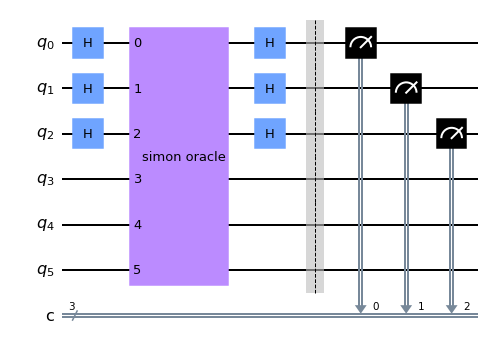
\includegraphics[width=\hsize]{qc_simon}
\end{center}

\end{columns}

\end{frame}

\begin{frame}{Algoritmo de Periodicidad de Simon}
Oráculo del circuito:
\begin{center}
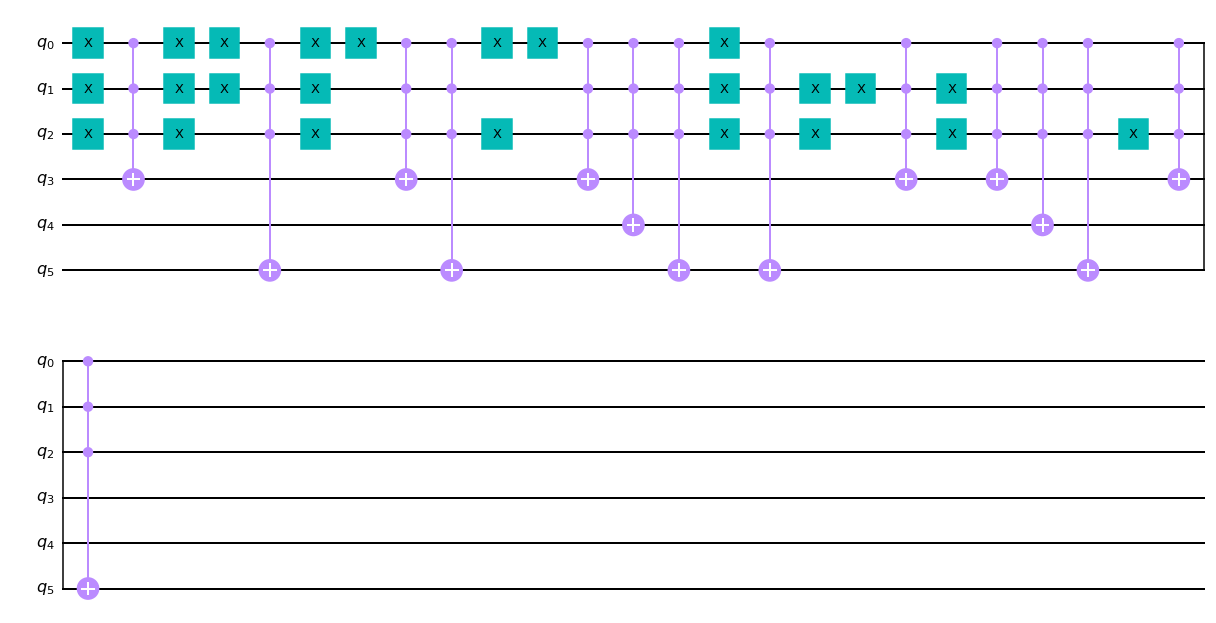
\includegraphics[height=0.8\vsize,width=\hsize]{simon_oracle}
\end{center}

\end{frame}


\begin{frame}{Algoritmo de Factorización de Shor}
\begin{itemize}[<+->]
\item Aplicaremos primero un procedimiento clásico para el algoritmo.

\item Aplicaremos después un procedimiento cuántico para el algoritmo. Lo usaremos para encontrar el orden $r$ de $x \modd N$.
\end{itemize}
\uncover<3->{
Estimación de Fase (Quantum Phase Estimation)
\begin{center}
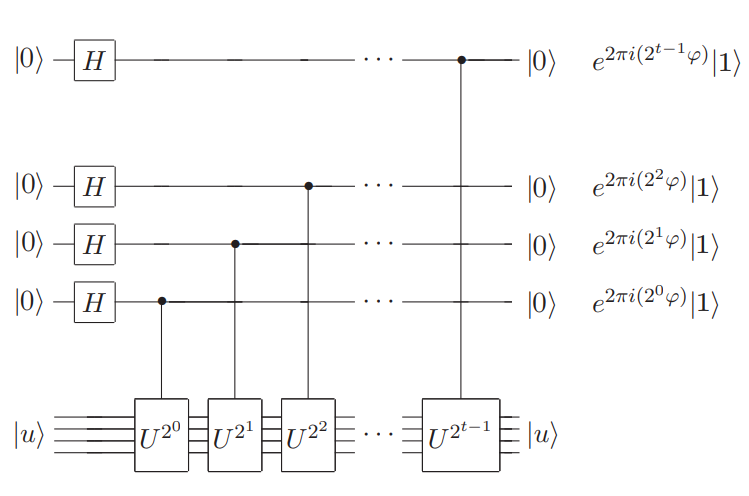
\includegraphics[scale=0.4]{orden}
\end{center}
El operador unitario que usaremos para hallar el orden es
\begin{equation}
U\ket{y} = \ket{x y \modd N}
\end{equation}
}

\end{frame}

\begin{frame}{Algoritmo de Factorización de Shor}
Transformada Cuántica de Fourier (Quantum Fourier Transformation)
\begin{center}
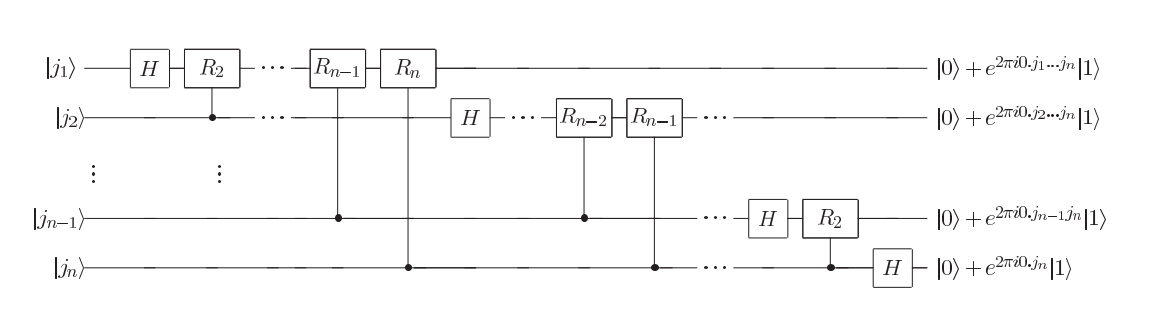
\includegraphics[scale=0.5]{qft}
\end{center}
Donde $R_k$ es la rotación que tiene por matriz:
\begin{equation}
R_k =
\begin{bmatrix}
1 & 0 \\
0 & e^{2\pi i/2^k}
\end{bmatrix}
\end{equation}

\end{frame}

\section{Ejecuciones de algoritmos}

\begin{frame}[fragile]{Ejecuciones de algoritmos}
Código en qiskit para el algoritmo de Grover:
\begin{columns}
\column{0.5\textwidth}
\begin{lstlisting}[language=Python]
#circuito_2
#solucion esperado: 110
gc = QuantumCircuit(4,3)
gc.h([0,1,2])
gc.initialize([0, 1], 3)
gc.h(3)
gc.barrier(range(4))
#iteración de grover
#oraculo
gc.x(0)
gc.mcx([0, 1, 2], 3)
gc.x(0)
gc.barrier(range(4))
\end{lstlisting}

\column{0.5\textwidth}
\begin{lstlisting}[language=Python]
#segunda simetría
gc.h([0,1,2])
gc.x([0,1,2])
gc.h(0)
gc.ccx(1,2,0)
gc.h(0)
gc.x([0,1,2])
gc.h([0,1,2])
gc.barrier(range(4))
gc.measure(range(3), range(3))
gc.draw('mpl')
\end{lstlisting}

\end{columns}
\end{frame}


\begin{frame}{Ejecuciones de algoritmos}

\only<1>{
Circuito cuántico de Grover implementado en qiskit:
\begin{center}
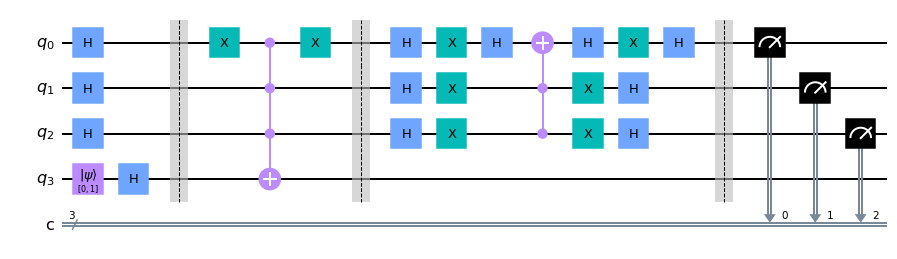
\includegraphics[scale=0.35]{qc_grover}
\end{center}}

\only<2>{
Simulación en un ordenador clásico:
\begin{center}
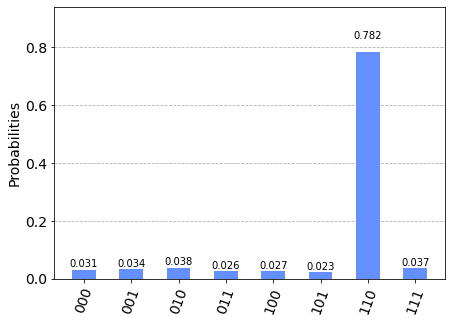
\includegraphics[scale=0.5]{grover_sim}
\end{center}}
\only<3>{
Ejecución en un ordenador cuántico:
\begin{center}
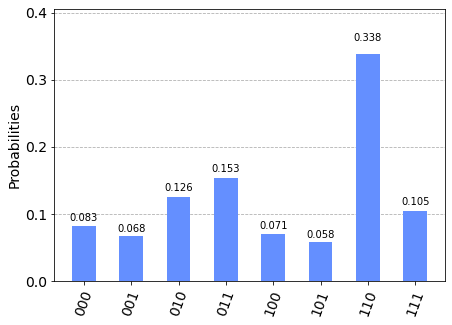
\includegraphics[scale=0.5]{grover_irl1}
\end{center}}
\only<4>{
Ejecución en un ordenador cuántico:
\begin{center}
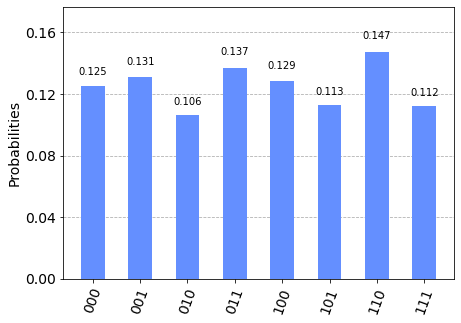
\includegraphics[scale=0.5]{grover_irl2}
\end{center}}

\end{frame}

\section{Conclusiones}

\begin{frame}{Conclusiones}
\begin{itemize}[<+->]
\item Se requiere conocimientos sobre álgebra lineal y producto tensorial para la computación cuántica.

\item A parte del área de estudio de cada algoritmo. Como el caso del algoritmo de factorización de Shor con la teoría de números.

\item Hay temas más complejos como la existencia de puertas universales.

\item Las implementaciones se han hecho con un número bajo de qubits.

\item La tecnología de hoy en día no permite una implementación totalmente funcional.

\end{itemize}

\end{frame}


\end{document}